\makeatletter
\def\input@path{{../../}}
\makeatother
\documentclass[../../main.tex]{subfiles}

\graphicspath{
	{../../img/}
	{../img/}
	{img/}
}

\begin{document}

\section{Гамма-функция Эйлера}

\emph{Эйлеровым интегралом второго рода} или \emph{$\Gamma$-функцией} 
называется
\begin{equation}
\label{lec13:1}
\Gamma(a) = \int\limits_0^{+\infty}e^{-x}x^{a-1}dx.
\end{equation}

\eqref{lec13:1} является НИЗОП-1 с подынтегральной функцией
$f(x, a) = e^{-x}x^{a-1}$, непрерывной на $\forall x > 0, \forall a \in \R$. 
Поэтому, отделяя в \eqref{lec13:1} особенности:
\begin{equation}
	\Gamma(a) = \underbrace{\int\limits_0^1e^{-x}x^{a-1}dx}_{\text{НИЗОП-2}} + 
	\underbrace{\int\limits_1^{+\infty}e^{-x}x^{a-1}dx}_{\text{НИЗОП-1}},
\label{lec13:2} 
\end{equation}
получаем, что:
\begin{enumerate}
\item 
$x \to + 0$; 
$\displaystyle f(x, a) \underset{x \to +0}\sim \left[ e^{-x} 
\underset{x \to +0} \to 1 \right] \sim \frac{1}{x^{1-a}}$
\item
$x \to +\infty$;
$0 \le f(x, a) = \dfrac{x^{a+1}}{e^x} \cdot \dfrac{1}{x^2} \le 
\dfrac{c}{x^2},\ 
c=const \ge 0$.
\end{enumerate}
Первое слагаемое сходится, когда $1 - a < 1 \implies a > 0$.
$\int\limits_1^{+\infty}\dfrac{c}{x^2}dx$ сходится по степенному признаку, 
следовательно, второе слагаемое НИЗОП-1 также сходится по признаку сравнения.
Т.~е. область существования (сходимости) для \eqref{lec13:1} будет $\forall a 
\in ]0, +\infty[$.

Нетрудно получить, что оба слагаемых в \eqref{lec13:2} в полученной области 
сходятся по признаку Вейерштрасса локально равномерно, т.~е.
$\Gamma(a) \overset{\forall \left[ \alpha, \beta \right] \in (0, 
+\infty)}{\rightrightarrows}$.
Значит, в своей области сходимости $\Gamma(a)$~--- непрерывная функция от $a$.

Учитывая далее, что для \eqref{lec13:2}
$\exists f'_a(x, a) = (e^{-x} x^{a-1})'_a = e^{-x}x^{a-1} \ln x$~--- 
непрерывная $\forall x>0,\forall a >0$, имеем:
\[
\int\limits_0^{+\infty} e^{-x} x^{a-1} \ln x\; dx
\overset{\forall \left[ \alpha, \beta \right] \in (0, 
	+\infty)}{\rightrightarrows}
\]
По теореме о дифференцировании НИЗОП-1 получаем, что
\[
\exists \Gamma'(a) = \int\limits_0^{+\infty} (e^{-x} x^{a-1})'_a dx = 
\int\limits_0^{+\infty} e^{-x} x^{a-1} \ln x\; dx 
\text{~--- непрерывная
$\forall a > 0$}.\]

Аналогичным образом по индукции $\forall k \in \N_0$ получаем
\[
\Gamma^{(k)}(a) = \ldots = \int\limits_0^{+\infty} e^{-x} x^{a-1} \ln^k x\; dx 
\]
$\Gamma^{(k)}(a)$ непрерывна $\forall a > 0$, т.~е. гамма-функция бесконечное 
число раз непрерывно дифференцируема.
При этом, т.~к. $\Gamma''(a) = \int\limits_0^{+\infty} e^{-x} x^{a-1} \ln^2 
x\; 
dx \ge 0$,
то график $\Gamma(a)$ будет выпуклым вниз. Имеем:
\begin{gather*}
\Gamma(1) = \int\limits_0^{+\infty} e^{-x} dx = [-e^{-x}]^{+\infty}_0 = 1
\\
\Gamma(2) = \int\limits_0^{+\infty} e^{-x} x\; dx = 
- \int\limits_0^{+\infty} x\; d(e^{-x}) = 
xe^{-x}\big|^{+\infty}_0 + \int\limits_0^{+\infty} e^{-x} dx = 
0 + 1 = 1
\end{gather*}
В таком случае, т.~к. $\Gamma(1) = \Gamma(2)$, то по теореме Ролля $\exists 
a_0 \in ]1, 2[$ такое, что $\Gamma'(a_0) = 0$, т.~е. $a_0$~--- 
стационарная 
точка (в данном случае она будет точкой минимума).

Приближенное вычисление дает $a_0 \approx 1,462$,\ \ 
$\Gamma(a_0) = \Gamma_{min} \approx 0.886$.

В результате получаем следующий график:

\begin{center}
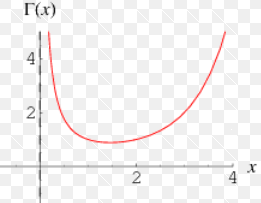
\includegraphics[scale = 0.8]{lec13_1} 
\end{center}

Интегрирование по частям дает:
\[
\Gamma(a) = \int\limits_0^{+\infty} e^{-x} d\left(\dfrac{x^a}{a}\right) =
 \dfrac{e^{-x}x^a}{a} \Big|^{+\infty}_0 - \int\limits_0^{+\infty} 
 \frac{x^a}{a} 
 d(e^{-x}) = 
 \frac{1}{a} \int\limits_0^{+\infty} e^{-x} x^a dx = \frac{\Gamma(a+1)}{a}
\implies\]\[\implies
\Gamma(a) = \frac{\Gamma(a+1)}{a},
\]
т.~е.
\begin{equation}
\Gamma(a+1) = a\Gamma(a),\ \forall a > 0
\label{lec13:3}
\end{equation}
При $a \to 0$ имеем
\[\Gamma(a) \sim \frac{\Gamma(1)}{a} = \dfrac{1}{a},\] т.~е. $a=0$~--- 
вертикальная асимптота.

Отсюда, учитывая, что $\Gamma(1) = 1\ \forall n \in \N$, получаем по индукции, 
что
\[\Gamma(n) = (n-1)\Gamma(n-1) = \cdots = (n-1) \cdot \ldots \cdot 2 \cdot 1 
\cdot 
\Gamma(1) = (n-1)!\]
Получили соотношение
\begin{equation}
\label{lec13:4}
\Gamma(n) = (n-1)!,\ \forall n \in \N.
\end{equation}
Из \eqref{lec13:4} можно рассматривать $\Gamma$-функцию как обобщение 
факториала. Кроме этого, также будем рассматривать значения $\Gamma(a)$ в 
полуцелых значениях аргумента, т.~е. $a = {n + \frac{1}{2}}, {n \in \N}$.
Последовательное применение \eqref{lec13:3} дает:
\[
\Gamma\left(n + \frac{1}{2}\right) = \left(n - 
\frac{1}{2}\right)\Gamma\left(n-\frac{1}{2}\right)=\ldots=
\left(n-\frac{1}{2}\right)\left(n-\frac{3}{2}\right)\ldots\cdot \frac{3}{2} 
\cdot \frac{1}{2} \cdot \Gamma\left(\frac{1}{2}\right) 
= 
\frac{(2n-1)!!}{2^n}\cdot \Gamma\left(\frac{1}{2}\right).
\]
Используя интеграл Эйлера-Пуассона, получаем:
\[
\Gamma\left(\frac{1}{2}\right) = \int\limits_0^{+\infty} e^{-x} 
x^{-\frac{1}{2}} dx = \left[\begin{array}{l}
x = t^2|_0^{+\infty} \\ dx = 2tdt
\end{array}
\right] = 
\int\limits_0^{+\infty} e^{-t^2} t^{-1} 2t\; dt = 2 \int\limits_0^{+\infty} 
e^{-t^2} dt 
= 2 \frac{\sqrt{\pi}}{2} = \sqrt{\pi},
\]
т.~е.
\begin{equation}
	\label{lec13:5}
	\begin{cases}
		\Gamma(n+\frac{1}{2}) = \frac{(2n-1)!!}{2^n} \sqrt{\pi},\ \forall n \in \N \\
		\Gamma(\frac{1}{2}) = \sqrt{\pi}
	\end{cases}
\end{equation}

\section{Бета-функция Эйлера}
\emph{$B$-функцией Эйлера} или \emph{эйлеровым интегралом первого рода} 
называется
\begin{equation}
	\label{lec13:6}
	B(a, b) = \int\limits_0^1x^{a-1}(1-x)^{b-1}dx
\end{equation}

Отделяя в \eqref{lec13:6} возможные особенности, получаем:
\begin{equation}
	\label{lec13:7}
	B(a, b) = \int\limits_0^{\frac{1}{2}} 
	x^{a-1} (1-x)^{b-1}dx + \int\limits_{\frac{1}{2}}^{1} 
	x^{a-1}(1-x)^{b-1}dx
\end{equation}

\begin{enumerate}
 \item $\displaystyle f(x, a, b) = x^{a-1}(1-x)^{b-1} \underset{x\to+0}\sim 
 \dfrac{1}{x^{1-a}}$.
 
  Первое слагаемое \eqref{lec13:7} будет сходиться при $1 - a < 1 \implies a > 
  0$.
  \item $f(x, a, b) \underset{x\to1-0}\sim \dfrac{1}{(1-x)^{1-b}}$.
  
  Второе слагаемое \eqref{lec13:7} сходится при $1-b < 1 \implies b > 0$.
\end{enumerate}

В итоге, областью существования (сходимости) \eqref{lec13:6} будет $a > 0, b > 
0$.
В дальнейшем основные свойства $B$-функции будем получать из соответствующих 
свойств $\Gamma$-функций. Для этого нам понабится

\begin{thm}[связь между $\Gamma$-функцией и $B$-функцией]
	\begin{equation}
	\label{lec13:8}
	\forall a > 0,\ \forall b>0 \implies B(a, b) = 
	\dfrac{\Gamma(a)\Gamma(b)}{\Gamma(a+b)}.
	\end{equation}
\end{thm}

\end{document}
